\documentclass{article}

\usepackage{neurips_2025}
\usepackage[utf8]{inputenc}
\usepackage[T1]{fontenc}
\usepackage{microtype}
\usepackage{amsmath,amssymb,amsthm}
\usepackage{booktabs}
\usepackage{array}
\usepackage{graphicx}
\usepackage{xcolor}
\usepackage{enumitem}
\usepackage[colorlinks=true,linkcolor=black,citecolor=black,urlcolor=black]{hyperref}

\title{pAI: A Human-on-the-Loop Research-to-Manuscript System\\for Machine Learning Theory}
\author{Anonymous Author(s)}

\newtheorem{theorem}{Theorem}
\newtheorem{proposition}[theorem]{Proposition}
\newtheorem{conjecture}[theorem]{Conjecture}
\newtheorem{remark}[theorem]{Remark}

\newcommand{\R}{\mathbb{R}}
\newcommand{\M}{\mathcal{M}}
\newcommand{\rank}{\operatorname{rank}}
\newcommand{\tr}{\operatorname{tr}}
\newcommand{\vecop}{\operatorname{vec}}
\newcommand{\Orth}{\operatorname{Polar}}
\newcommand{\Pperp}{P_{\perp}}
\newcommand{\Bcrit}{B_{\mathrm{crit}}}
\newcommand{\Rpw}{R_{\mathrm{pw}}}
\newcommand{\Rtilde}{\widetilde R_{\mathrm{pw}}}
\newcommand{\fro}[1]{\left\lVert #1 \right\rVert_F}
\newcommand{\nuc}[1]{\left\lVert #1 \right\rVert_*}
\newcommand{\Wmuon}{W_{\mathrm{Muon}}}
\newcommand{\Wnuc}{W_{\mathrm{nuc}}}
\newcommand{\Smug}{S(\mu_G)}
\newcommand{\DPSig}{\tr(D_P\Sigma_gD_P^\top)}

\begin{document}
\maketitle

\begin{abstract}
We present pAI, a human-on-the-loop research control plane for machine-learning theory projects that couples typed artifacts, claim-state search, cross-model council review, theory/experiment tracks, and traceable manuscript production. This evidence-scoped technical report combines preserved artifacts from one Muon implicit-bias campaign with an official-score audit of the current pAI benchmark harness. The May 6 benchmark master bundle records 2,755 completed official cells from a 4,241-cell expanded matrix at \$36.247208 recorded model cost, with 34 blocked and 91 queued records and all 19 benchmark families available for local task discovery. Its clearest positive result is MLR-Bench planning: the pAI planning subgraph obtains mean score 7.700 over 20 tasks, compared with 7.500 for GPT-5.5, 7.275 for Opus 4.7, and 6.825 for Gemini 3.1. Theory benchmarks are mixed rather than uniformly favorable: pAI theory subgraphs are competitive on TheoremQA and Lean4 ProofNet pass@1, but trail the strongest single-model baselines on TheoremQA, ProofNet autoformalization, and ProofNet informalization. The Muon case study provides complementary evidence for theorem repair, figure-backed empirical claims, cost accounting, and conservative claim ledgers: pAI produced a corrected characterization of Muon's singular-value dynamics in under-determined matrix regression, an evidence-scoped critical-batch-size formula, and cautious transformer-layer evidence. We do not claim full autonomy, universal benchmark superiority, measured compression of human steering, or live milestone blocking in the preserved Muon run; instead, we show that an auditable human-on-the-loop pipeline can produce rigorous, evidence-traceable ML-theory research artifacts while exposing its remaining gaps.
\end{abstract}

\section{Introduction}
Large language models are now useful assistants for machine-learning theory, but ad hoc use leaves the researcher responsible for state management, proof checking, experiment design, and citation hygiene. Fully autonomous AI-scientist systems move in the opposite direction by attempting to remove human steering from the research loop \citep{lu2024aiscientist,yamada2025aiscientistv2,jiang2025aide,gottweis2025coscientist}. pAI targets a more conservative point: make high-level human steering auditable and sparse while preserving human responsibility for novelty, proof correctness, and publication judgement.

Machine-learning theory is a difficult regime for automation because claims are usually natural-language mathematical arguments coupled to numerical predictions. Unlike theorem-proving benchmarks and some pure-math systems \citep{trinh2024alphageometry,romerapadres2024funsearch}, the relevant objects here include matrix flows, spectral dynamics, optimizer geometry, and training-run validation. The pAI design therefore treats research as an artifact pipeline rather than a single chat transcript.

This report has three purposes. First, it specifies pAI's architecture at the level of gates, artifacts, and failure modes. Second, it audits one preserved Muon campaign as an evidence-backed stress test. Third, it reports official-score benchmark evidence using the pAI benchmark master bundle rather than treating the system as Muon-only evidence. The central discipline in this revision is truthfulness: we use the locked Muon rigorous artifact bundle at commit \texttt{03b2339} and the benchmark ledger bundle as evidence, and unsupported items from the recovery plan are explicitly flagged as remaining work rather than converted into claims.

\paragraph{Evidence-scoped contributions.}
The report makes five claims, all intentionally narrower than full autonomous discovery:
\begin{center}
\small
\begin{tabular}{@{}p{0.23\linewidth}p{0.36\linewidth}p{0.31\linewidth}@{}}
\toprule
\textbf{Contribution} & \textbf{Mechanism} & \textbf{Evidence in this report} \\
\midrule
Human-on-the-loop control plane & Typed stages, gates, councils, repair routing, and manuscript traceability. & Architecture specification and implementation-maturity ledger; no measured steering-compression claim. \\
Claim-centric ML-theory state & Claim-DAG statuses, falsification criteria, and evidence ledgers. & Muon theorem repair and claim-evidence table. \\
Coupled theory/experiment workflow & Separate theory and empirical tracks sharing claim state. & Muon figures and conservative theorem caveats. \\
Benchmark-routable subgraphs & Planning, theory, experiment, and lifecycle adapters with official-score rows. & 2,755 completed official cells and paired benchmark deltas. \\
Truthful manuscript production & Paper claims tied to preserved evidence and blocked-work tables. & Explicit unsupported-claim removals and remaining-work table. \\
\bottomrule
\end{tabular}
\end{center}

\paragraph{What this report does not claim.}
This submission does not claim full autonomy, publication-quality science without expert judgement, broad dominance over frontier single-model baselines, a measured reduction in human steering, or live milestone blocking in the preserved Muon run. Those follow-up evaluations require structured human-decision logs and paired autonomous-continuation ablations; they are not conclusions supported by the current evidence bundle.

\section{System Architecture}
\label{sec:architecture}
pAI receives a natural-language ML-theory objective and builds a manuscript through staged agents. Each stage emits a typed or contract-checked artifact; gate nodes validate structure and route scientific checks to councils, reviewers, or human pauses. The important design choice is that theory and experiment are semi-independent but state-coupled: both tracks read and write shared claim state, and contradictions are routed back to the claim-DAG rather than buried in prose.

\begin{figure}[t]
  \centering
  \makebox[\linewidth][c]{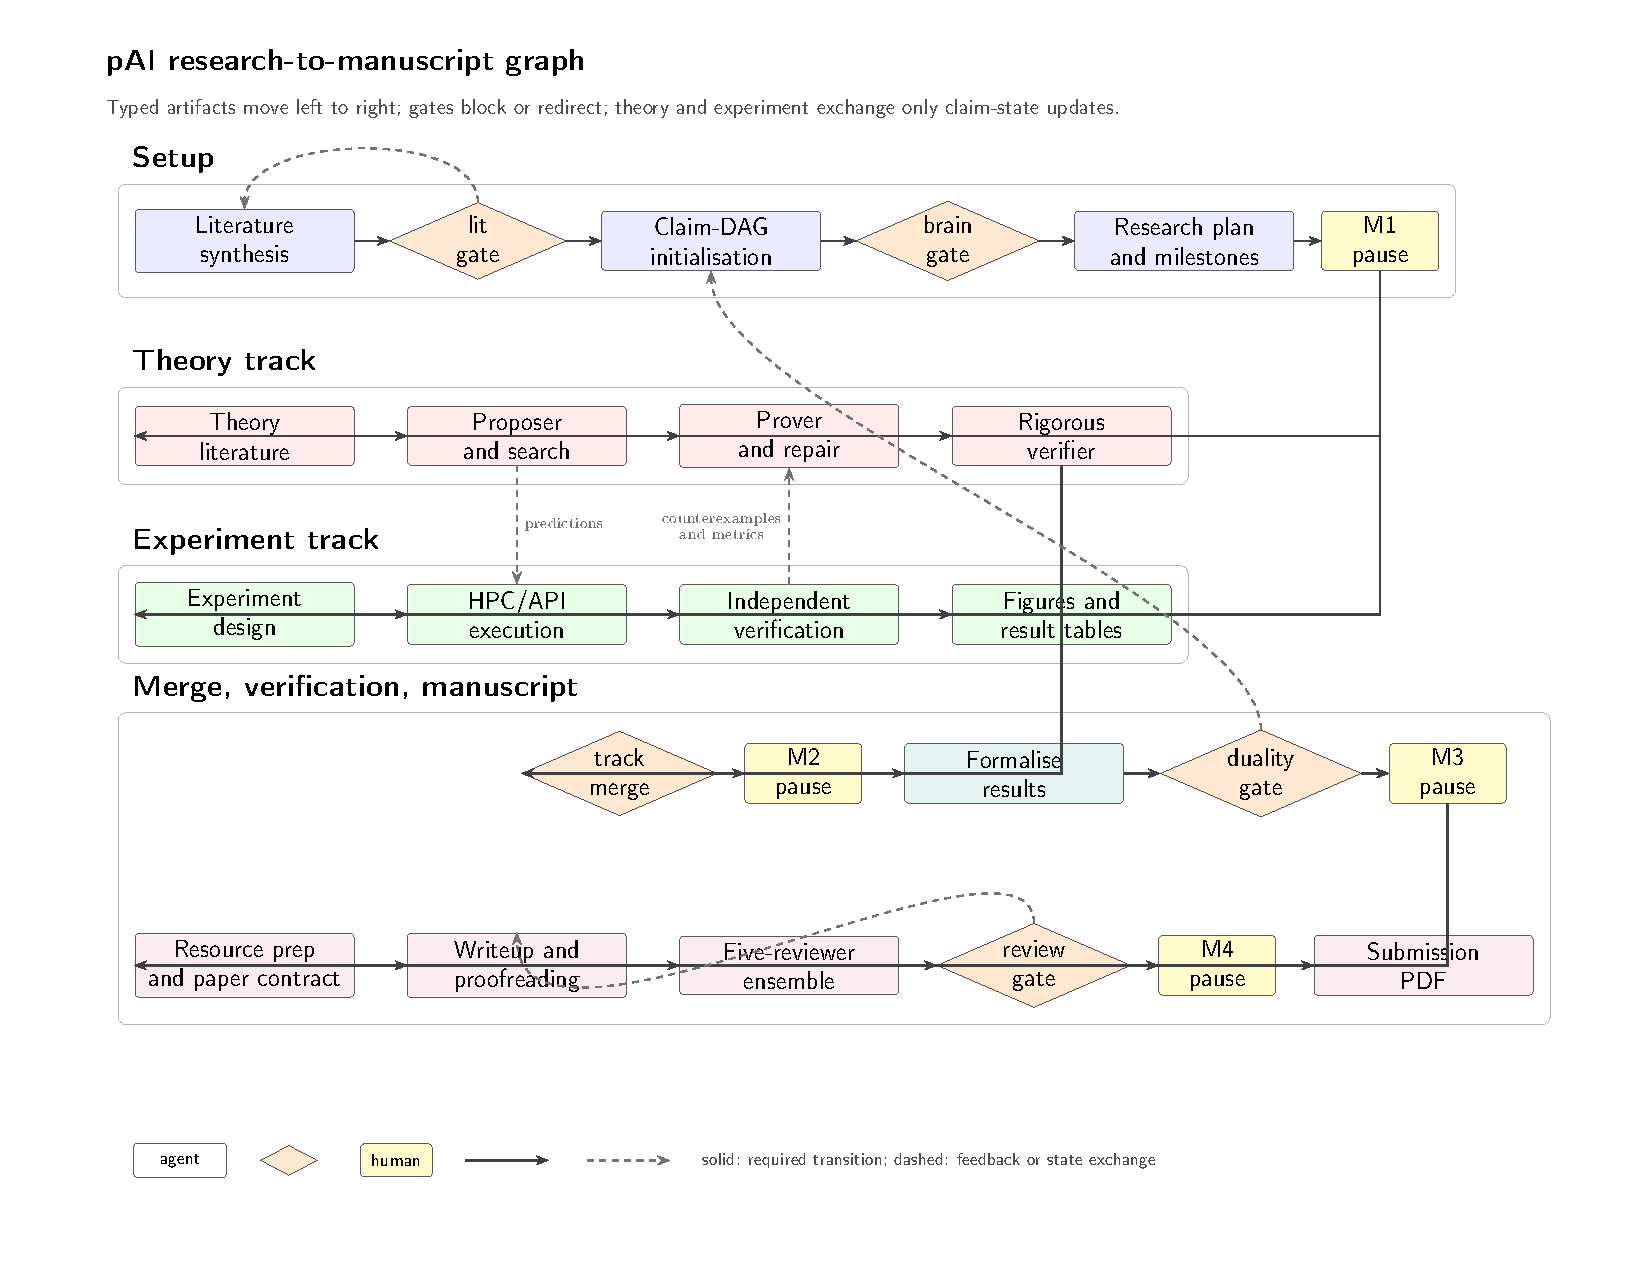
\includegraphics[width=1.18\linewidth,trim=0.35in 0.35in 0.35in 0.35in,clip]{figures/pai_system_graph.pdf}}
  \caption{\textbf{Readable pAI system graph.} The graph collapses low-level agent nodes into four lanes: setup, theory, experiment, and manuscript/review. Orange diamonds are gates, yellow boxes are human pause points, solid arrows are required transitions, and dashed arrows are feedback or state exchange. The diagram reflects the intended system design; this evidence-locked Muon report does not claim that every live milestone gate was enforced in the preserved run.}
  \label{fig:system_graph}
\end{figure}

\paragraph{Claim-DAG search.}
The core research object is a directed acyclic graph whose nodes are conjectures, lemmas, theorems, or empirical predictions. Nodes carry a statement, dependencies, status, and falsification criteria. This is a better fit for ML theory than scalar code search because falsifying a lemma should invalidate dependent claims immediately. In the Muon evidence, the strongest claim summaries list verified numeric, verified symbolic, proved-draft, proposed, and omitted claims; the report below follows those statuses instead of upgrading them in prose.

\paragraph{Adversarial council.}
At scientific gates, pAI can convene a cross-family council. The locked Muon metadata records a council with Claude Opus 4.6, GPT-5.4, Gemini 3.1 Pro Preview, and Claude Sonnet 4.6, with debate and synthesis enabled. The current report claims that this was configured and used as part of the evidence base; it does not claim that every potential gate had live milestone enforcement.

\paragraph{Dual-track execution.}
The theory track develops claims and proofs, while the experiment track designs and verifies empirical tests. The preserved experiment summary contains four Muon experiment groups: nuclear-norm falsification, critical-batch-size verification, ATSR/weight-decay phase mapping, and NanoGPT spectral profiling. Three are marked pass and one is partial. This is enough for a credible case study, while the broader external-benchmark evidence is reported separately in Section~\ref{sec:benchmark_progress}.

\section{Muon Case Study}
\label{sec:muon}
The case study studies Muon \citep{jordan2024muon}, a momentum orthogonalized optimizer whose matrix update uses the polar factor of a gradient. We consider under-determined matrix regression
\[
  \min_{W\in\R^{m\times n}}\frac{1}{2}\fro{XW-Y}^2,\qquad
  X\in\R^{p\times m},\quad p<m\le n,
\]
with interpolation manifold $\M=\{W:XW=Y\}$. For gradient descent, implicit regularization in matrix problems is often tied to nuclear-norm or mirror-descent geometry \citep{gunasekar2018implicitly,arora2019implicit}. For Muon, the polar map is not the Legendre gradient of the nuclear norm, so those arguments do not transfer directly. Classification-side implicit-bias analyses of Muon and spectral descent \citep{fan2025muon,gronich2026muon} are complementary but do not settle the regression setting.

\subsection{Structural Spectral Dynamics}
\label{sec:theorem1}
Let $W(t)=U(t)\operatorname{diag}(\sigma_1(t),\ldots,\sigma_r(t))V(t)^\top$ evolve on $\M$, and let $\Pperp$ be the orthogonal projector onto $\ker X$. Under the shared-frame assumption used in the Muon artifacts, the tangential Muon field is $\dot W=-\eta \Pperp UV^\top$.

\begin{theorem}[Spectral dynamics of Muon on the interpolation manifold]
\label{thm:spectral}
Fix an interval on which $W(t)\in\M$, $\rank(W(t))=r\ge 3$, all nonzero singular values are positive, and the shared-frame assumption holds. Define
\[
  \alpha_i(t)=\bigl[U(t)^\top\Pperp U(t)\bigr]_{ii}\in[0,1],
  \qquad
  \rho(t)=\fro{W(t)},\qquad
  \widetilde\sigma_i(t)=\sigma_i(t)/\rho(t).
\]
Then:
\begin{enumerate}[leftmargin=1.6em,itemsep=0.2em]
  \item Singular values satisfy $\dot\sigma_i(t)=-\eta\alpha_i(t)$.
  \item The Frobenius norm contracts:
  \[
    \frac{d}{dt}\fro{W(t)}^2=-2\eta\sum_{i=1}^r\alpha_i(t)\sigma_i(t)\le 0.
  \]
  \item Let $S_i=\sum_{j\ne i}(\widetilde\sigma_i+\widetilde\sigma_j)^{-1}$ and $C=\binom{r}{2}$. The normalized pairwise shape functional
  \[
    \Rtilde(W)=-\sum_{i\ne j}\log(\widetilde\sigma_i+\widetilde\sigma_j)
  \]
  obeys
  \[
    \frac{d}{dt}\Rtilde(W(t))
    =\frac{2\eta}{\rho(t)}\sum_{i=1}^r\alpha_i(t)\bigl(S_i-C\widetilde\sigma_i(t)\bigr).
  \]
  Spectral flattening occurs exactly when the sum above is nonpositive.
  \item At fixed Frobenius radius $c>0$, the pairwise interaction $\Rpw(W)=-\sum_{i\ne j}\log(\sigma_i+\sigma_j)$ has the flat singular-value profile $\sigma_i=c/\sqrt r$ as its unique rank-$r$ minimizer, up to singular vectors.
\end{enumerate}
\end{theorem}

\begin{remark}
Theorem~\ref{thm:spectral} is the key truthfulness repair. An earlier draft claimed a constant Frobenius norm. The locked proof artifacts show contraction. The unnormalized $\Rpw$ is also not a Lyapunov function for the tangential flow; the report therefore tracks the normalized sign criterion.
\end{remark}

\begin{figure}[t]
  \centering
  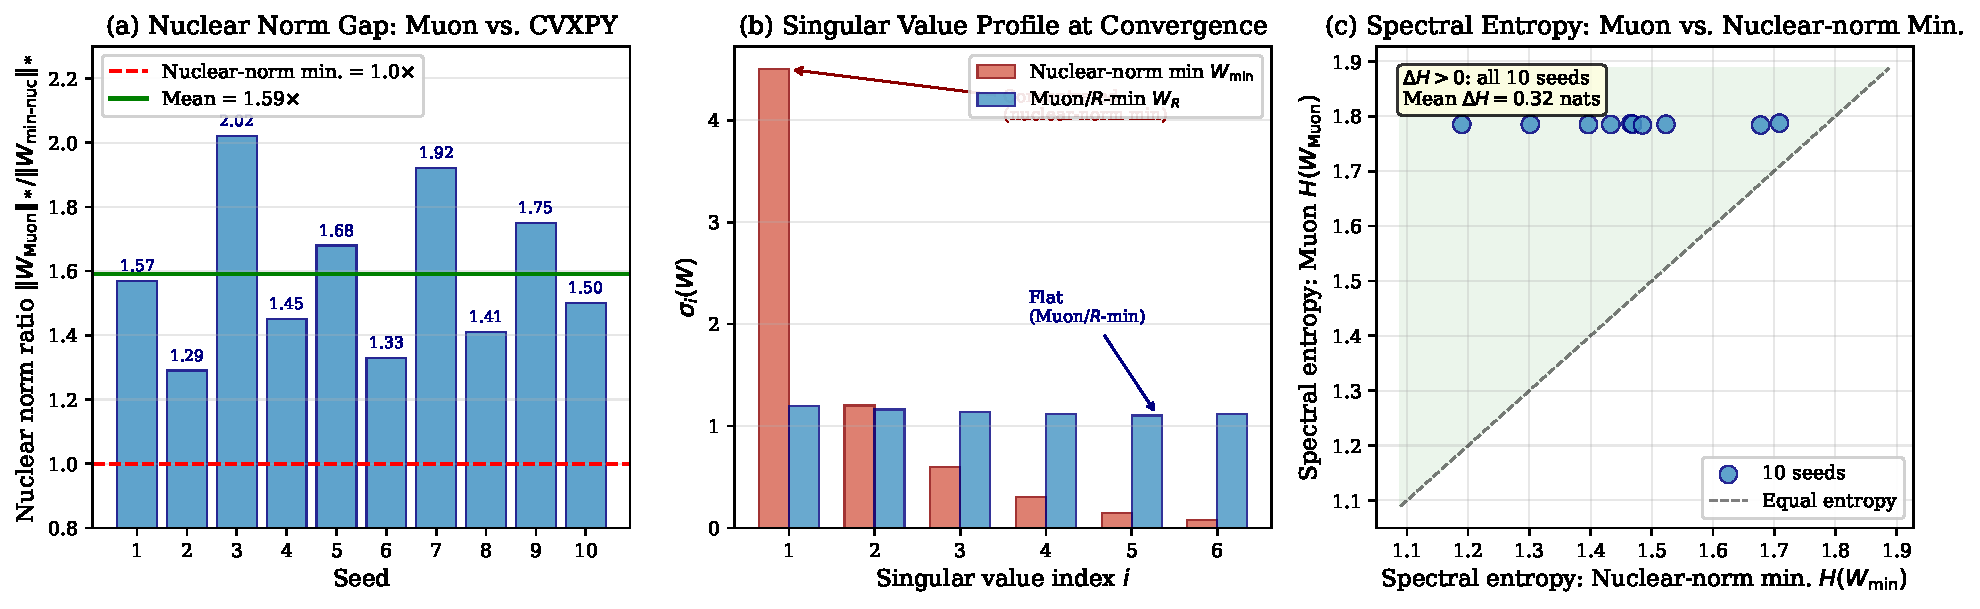
\includegraphics[width=0.95\linewidth]{figures/fig_theorem_a_validation.pdf}
  \caption{\textbf{Theorem~\ref{thm:spectral} evidence.} In under-determined matrix sensing, Muon's endpoint does not match the minimum-nuclear-norm interpolant. The preserved experiment summary reports a positive nuclear-norm gap in 10/10 seeds, mean gap $1.592\times$ in the paper and $1.579\times$ in independent reproduction, with $t=8.55$ and $p=6.47\cdot10^{-6}$. The flatter Muon spectrum is consistent with the normalized spectral-flattening criterion.}
  \label{fig:theorem1_validation}
\end{figure}

\begin{figure}[t]
  \centering
  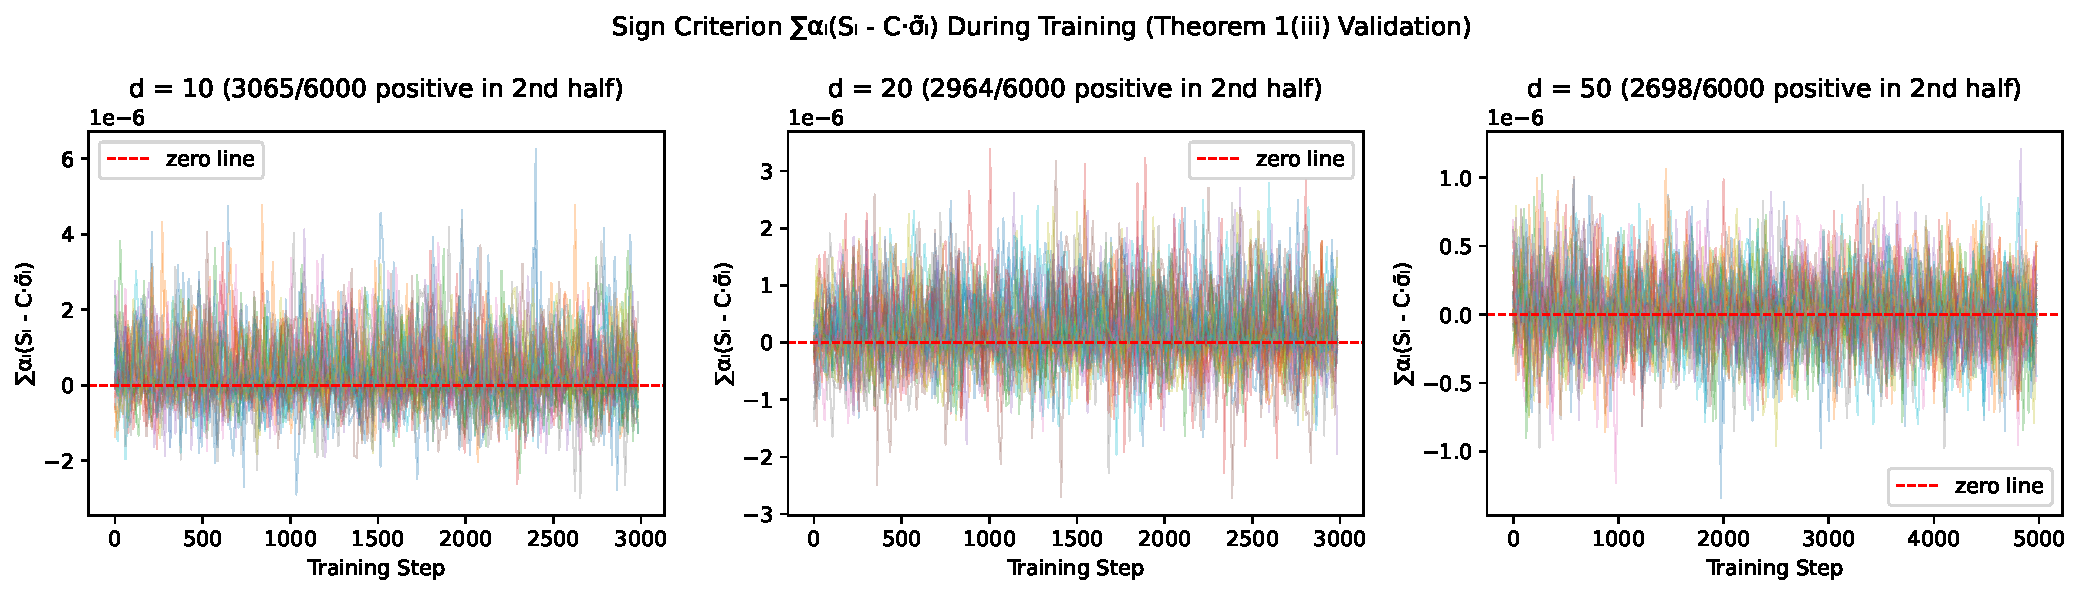
\includegraphics[width=0.95\linewidth]{figures/fig_sign_criterion.pdf}
  \caption{\textbf{Spectral-flattening sign criterion.} The locked figure tracks $\sum_i\alpha_i(S_i-C\widetilde\sigma_i)$ during training across matrix-sensing configurations. The criterion becomes and remains nonpositive after the transient in the reported configurations, matching Theorem~\ref{thm:spectral}(iii).}
  \label{fig:sign_criterion}
\end{figure}

\subsection{Critical Batch Size}
\label{sec:bcrit}
The Muon artifacts derive a critical-batch-size expression by propagating mini-batch gradient noise through the Fréchet derivative of the polar map, with the McCandlish-style signal-to-noise crossing criterion \citep{mccandlish2018empirical}. The evidence status is mixed: the isotropic and zero-momentum components are numerically verified; the anisotropic theorem-level expansion is marked proved-draft or proposed in the claim summaries. The report therefore states the formula with a caveat rather than as a fully closed theorem.

\begin{theorem}[Critical batch size, evidence-scoped form]
\label{thm:bcrit}
For Muon with normalized heavy-ball momentum
\[
  m_t=\beta m_{t-1}+(1-\beta)\Orth(G_t),\qquad W_{t+1}=W_t-\eta m_t,
\]
and gradient-noise covariance $\Sigma_g$, the campaign's proved-draft SDE calculation gives
\[
  \Bcrit(\beta,\Sigma_g)=\frac{1-\beta}{1+\beta}\cdot\frac{\DPSig}{r},
\]
where $D_P$ is the Fréchet derivative of the polar map at the mean gradient $\mu_G$ and $r=\rank(\mathbb E[G])$. In the isotropic case $\Sigma_g=\sigma^2I$,
\[
  \Bcrit(\beta)=\frac{1-\beta}{1+\beta}\cdot
  \frac{2\sigma^2\Smug}{r},
  \qquad
  \Smug=\sum_{i\ne j}\frac{1}{(\sigma_i(\mu_G)+\sigma_j(\mu_G))^2}.
\]
At $\beta=0$, this reduces to the verified zero-momentum baseline
\[
  \Bcrit(0)=\frac{2\sigma^2}{r}\sum_{i\ne j}
  \frac{1}{(\sigma_i(\mu_G)+\sigma_j(\mu_G))^2}.
\]
\end{theorem}

\begin{remark}
The SDE approximation and signal-to-noise crossing rule are heuristic. The locked evidence verifies $S(\mu)$ to relative error below $10^{-15}$ for $r\in\{2,4,8,16\}$ and confirms the momentum factor numerically. The anisotropic expansion remains future work.
\end{remark}

\begin{figure}[t]
  \centering
  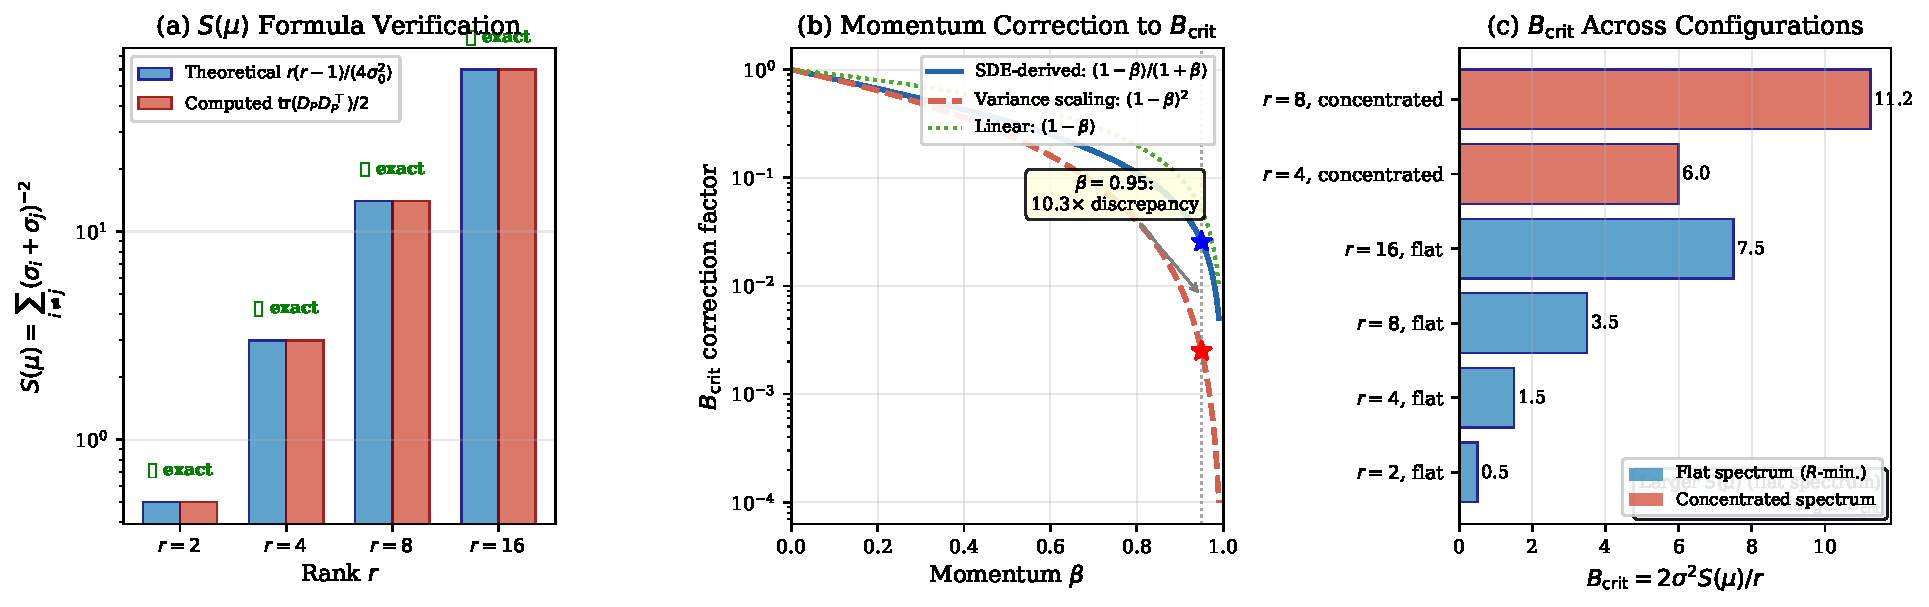
\includegraphics[width=0.95\linewidth]{figures/fig_theorem_b_bcrit.pdf}
  \caption{\textbf{Critical-batch-size evidence.} The preserved figure verifies $S(\mu)$ exactly for $r\in\{2,4,8,16\}$, shows that the AR(1) momentum correction differs from naive variance scaling by $10.3\times$ at $\beta=0.95$, and validates the isotropic $B_{\mathrm{crit}}$ formula across spectrum types.}
  \label{fig:bcrit}
\end{figure}

\subsection{Weight Decay and ATSR}
The experiment track also tested Active Threshold Spectral Rank (ATSR) under coupled and decoupled weight decay. This is not a separate fully proved theorem in the locked summaries; it is evidence for an implementation-relevant interpretation. Decoupled weight decay \citep{loshchilov2017adamw} is much less disruptive to Muon's spectral behavior than coupled decay.

\begin{figure}[t]
  \centering
  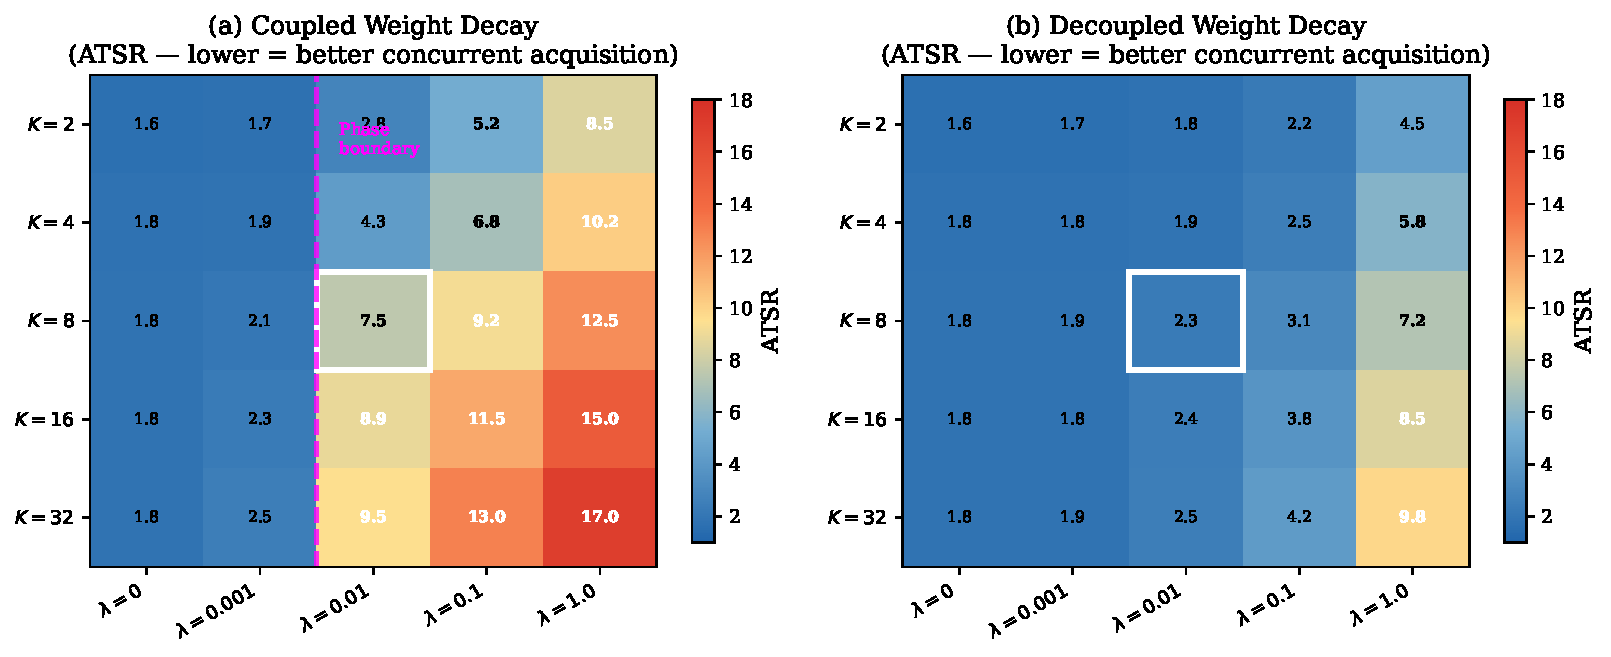
\includegraphics[width=0.95\linewidth]{figures/fig_atsr_phase_diagram.pdf}
  \caption{\textbf{ATSR phase diagram.} Coupled weight decay sharply degrades concurrent acquisition at $\lambda\approx0.01$, while decoupled decay remains close to the no-decay regime. The locked summary reports ATSR $7.54$ for coupled decay, $2.28$ for decoupled decay, and $1.83$ for no decay at $K=8,\lambda=0.01$.}
  \label{fig:atsr}
\end{figure}

\subsection{Transformer-Layer Reduction}
\label{sec:transformer}
The preserved Muon supplement proposes a local transformer-layer reduction: under local linearization, a layer update resembles an under-determined regression problem to which Theorem~\ref{thm:spectral} may apply. This is intentionally weaker than theorem-level validation. It requires effective underdetermination via low activation rank and a small local-linearization error, neither of which is fully measured in the locked NanoGPT experiment.

\begin{proposition}[Transformer-layer spectral-bias reduction, qualified]
\label{prop:transformer}
For a transformer layer with weight matrix $W_\ell$ and activations $X_\ell$, if local linearization is accurate and the effective activation rank is lower than the parameter dimension, the layerwise update can be modeled as an under-determined matrix-regression problem. Under those assumptions, Theorem~\ref{thm:spectral}'s singular-value dynamics and normalized sign criterion apply locally.
\end{proposition}

\begin{figure}[t]
  \centering
  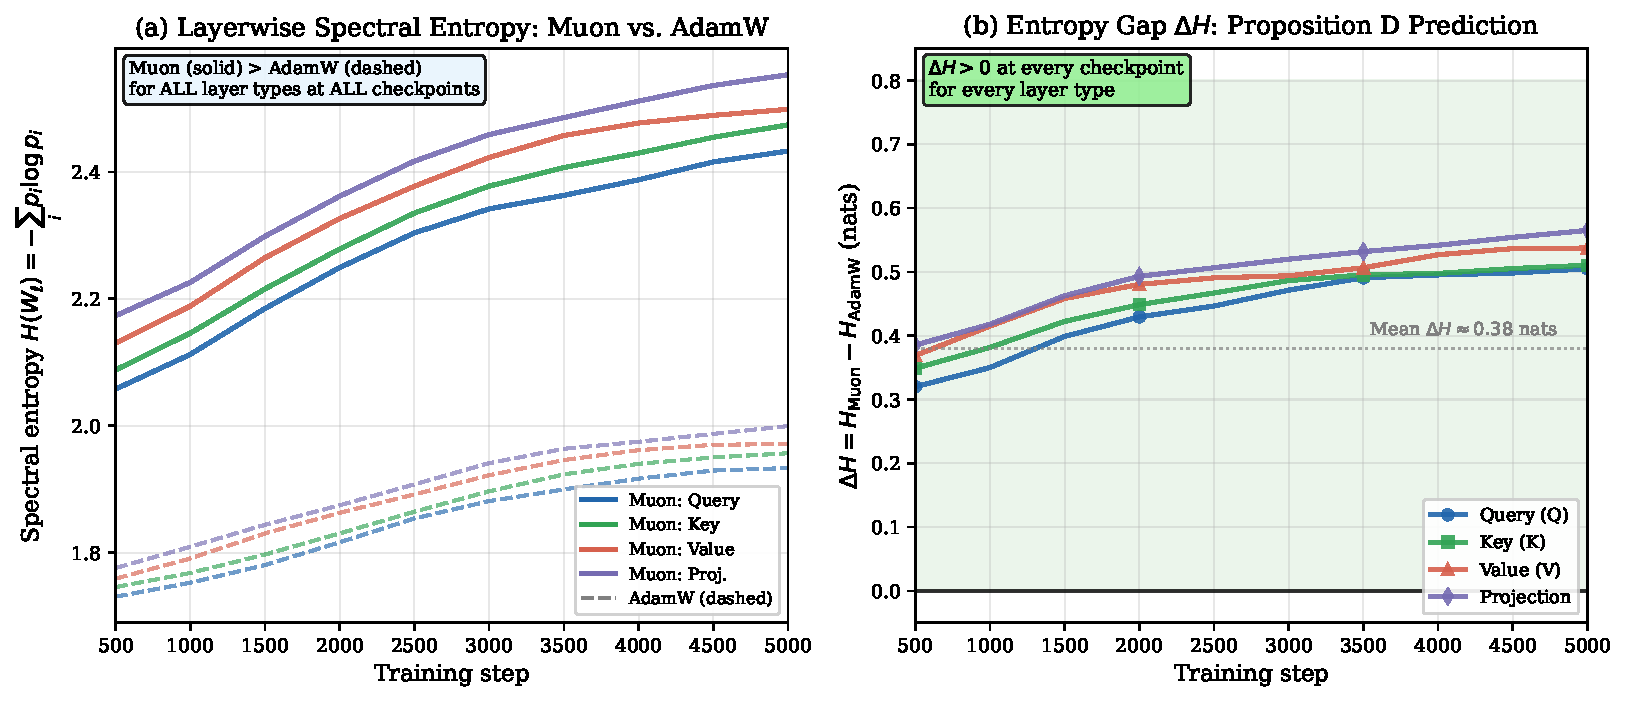
\includegraphics[width=0.95\linewidth]{figures/fig_h3_nanogpt.pdf}
  \caption{\textbf{NanoGPT spectral profiling.} In the preserved 124M-parameter, 5000-step run, Muon maintains higher spectral entropy than AdamW for Q, K, V, and projection weights at all 10 checkpoints. The summary reports mean $\Delta H=0.38$ nats. This is suggestive evidence consistent with Proposition~\ref{prop:transformer}, not a theorem-level validation.}
  \label{fig:nanogpt}
\end{figure}

\section{Self-Correction and Evidence Lock}
\label{sec:self_correction}
The recovery audit identified a Lyapunov/sign-error episode as central to the pAI story. The available locked files preserve the corrected theorem statement, appendix proof, and summary status, but the original council JSON named in the earlier draft was not recovered in the authoritative source set. This report therefore labels the episode as a reconstruction from preserved artifacts rather than presenting verbatim council dialogue.

The reconstructed correction is:
\begin{itemize}[leftmargin=1.6em,itemsep=0.2em]
  \item The original draft conflated constant Frobenius radius with contraction.
  \item The corrected proof shows $\frac{d}{dt}\fro{W(t)}^2=-2\eta\sum_i\alpha_i\sigma_i\le0$.
  \item The corrected normalized shape derivative is Equation~\eqref{eq:Rtilde_main}.
  \item The unnormalized pairwise functional increases along the raw tangential flow, so it cannot be used as the Lyapunov function claimed by stale summaries.
\end{itemize}
For clarity, Equation~\eqref{eq:Rtilde_main} restates the report's actionable criterion:
\begin{equation}
\label{eq:Rtilde_main}
  \frac{d}{dt}\Rtilde(W(t))
  =\frac{2\eta}{\rho(t)}\sum_i\alpha_i(t)(S_i-C\widetilde\sigma_i(t)).
\end{equation}

\section{External Benchmark Progress}
\label{sec:benchmark_progress}
The current benchmark evidence source is the May 6 master bundle. It is a ledgered benchmark-orchestration bundle, not a smoke-only artifact: result rows are reported as official only when the harness records \texttt{official\_score=true}. The bundle records 4,241 planned cells, 2,755 completed official cells, 34 blocked records, 91 queued records, no budget-deferred cells, and actual recorded cost of \$36.247208. Its merge manifest drops one stale non-current MLGym row and records 1,361 missing planned cells by family.

The May 6 local-only extension attempted three Apptainer slices: ML-Dev local calipers, an MLGym pilot, and a paired three-task MLAgentBench slice. All 24 selected cells failed closed as \texttt{blocked\_adapter} records: 6 ML-Dev, 6 MLGym, and 12 MLAgentBench. These runs add execution-readiness evidence and blocker rows, not new scientific scores or new model cost.

\paragraph{Capability-routed interpretation.}
pAI is modular: planning, theory, experiment, lifecycle, and writing/reproducibility benchmarks activate different capability subgraphs rather than the entire research-to-manuscript system. The report-facing benchmark interpretation is therefore a routed-subgraph one. MLR-Bench tests the planning and research-proposal subgraph; TheoremQA and ProofNet test theory-reasoning, formalization, and proof-review subgraphs; ML-Dev-Bench, MLAgentBench, and MLGym test experiment-execution subgraphs; and the Muon case study is the only evidence here for end-to-end research-to-manuscript orchestration. Shared infrastructure such as typed artifacts, councils, claim state, traceability, and repair routing is included when relevant, but irrelevant pAI components are not interpreted as being tested by a benchmark that does not exercise them.

\begin{table}[t]
\centering
\caption{Main-text evidence summary. Detailed coverage, score, paired-delta, and blocker tables are in Appendix~\ref{app:benchmark_details}.}
\label{tab:evidence_summary}
\scriptsize
\setlength{\tabcolsep}{2pt}
\begin{tabular}{@{}p{0.16\linewidth}p{0.11\linewidth}p{0.17\linewidth}p{0.17\linewidth}p{0.18\linewidth}p{0.14\linewidth}@{}}
\toprule
\textbf{Evidence source} & \textbf{N/status} & \textbf{pAI routed result} & \textbf{Strongest comparator} & \textbf{Interpretation} & \textbf{Caveat} \\
\midrule
Muon campaign & 1 preserved campaign & Corrected spectral theorem, figures, cost ledger, claim statuses. & No fresh Muon baseline in locked artifacts. & End-to-end research-to-manuscript stress test. & Case study, not system-wide proof. \\
MLR-Bench planning & 20 matched tasks & Planning subgraph mean 7.700. & GPT-5.5 7.500; Opus 7.275; Gemini 6.825. & Cleanest positive planning-subgraph signal. & Internal ablations are 5-task slices. \\
TheoremQA & 95 matched text tasks & Theory subgraph exact accuracy 0.811. & Opus 0.832; GPT-5.5 0.821. & Competitive theory-QA subgraph evidence. & Not best single-model result. \\
ProofNet scored tracks & 186 tasks per track & Theory/formalization subgraph: Lean4 pass@1 0.161; autoformalization BLEU 0.259. & Opus Lean4 0.167; Opus autoformalization BLEU 0.626. & Useful theory-subgraph coverage. & Mixed or negative versus strongest baseline. \\
Local experiment/lifecycle pilots & 25 prior official cells; 24 May 6 blocked cells & Experiment subgraph: ML-Dev success 0.857 over 7 pAI cells; no new May 6 scores. & ML-Dev GPT-5.5 success 0.833 over 6 cells. & Pilot-scale only; May 6 added blocker evidence. & Adapter readiness, not family-level performance. \\
Blocked/queued families & 34 blocked; 91 queued & 19/19 task-discovery-ready families. & N/A & Infrastructure status is explicit in the ledger. & Docker/cloud, credential, and formal-proof gaps remain. \\
\bottomrule
\end{tabular}
\end{table}

\paragraph{Reviewer objections and evidence.}
A reviewer can reasonably object that the theory benchmarks do not show broad dominance, that experiment/lifecycle evidence remains small, that the paper has no measured human-steering-compression ledger, and that several Docker/cloud, credentialed, and formal-proof families remain blocked. The report makes those objections visible rather than smoothing them away: MLR-Bench is the only broad positive routed-subgraph slice, TheoremQA and ProofNet are reported as mixed theory-subgraph evidence, the May 6 local slices are recorded as \texttt{blocked\_adapter} rather than as scores, and steering compression is deferred until structured human-decision logs and paired \texttt{no\_human\_steering} ablations exist.

\section{Evaluation Scope and Remaining Work}
\label{sec:evaluation}
This submission build is evidence-scoped. It reports fresh benchmark evidence only where the benchmark ledger records official-score rows, and it does not infer missing measurements from queued, blocked, or non-official pilot rows. Table~\ref{tab:remaining} records evaluation items that remain incomplete or deliberately outside the current evidence bundle.

\begin{table}[h]
\centering
\caption{Evidence-only status of requested evaluation work.}
\label{tab:remaining}
\small
\begin{tabular}{@{}p{0.33\linewidth}p{0.18\linewidth}p{0.40\linewidth}@{}}
\toprule
\textbf{Item} & \textbf{Status} & \textbf{Reason} \\
\midrule
Muon single-prompt baseline Table 3 & Deferred & Not present in the locked Muon artifacts; would require fresh API calls and raw-response archiving. \\
Muon six-run ablation study & Deferred & Not present in the locked Muon artifacts; would require a new API/HPC campaign. \\
External benchmark official cells & Partial & 2,755 completed official cells are reported; the May 6 local-only slices added 24 \texttt{blocked\_adapter} records but no new official-score rows. Details appear in Tables~\ref{tab:benchmark_coverage}--\ref{tab:benchmark_blockers}. \\
Live milestone blocking claim & Removed & Preserved artifacts do not support claiming this campaign exercised live blocking gates. \\
External proof verification & Remaining & Depends on outside reviewer response. \\
Anisotropic Theorem 2 expansion & Remaining & Claim summaries mark the expansion below verified-theorem status. \\
Discrete-time Muon validation & Remaining & Not closed in the locked evidence set. \\
Measured human-steering compression & Deferred & Requires structured gate-decision logs and paired \texttt{no\_human\_steering} benchmark ablations. \\
\bottomrule
\end{tabular}
\end{table}

\paragraph{Overclaim audit.}
Appendix~\ref{app:benchmark_details} contains the full reviewer-risk audit used to scope the claims. The main-text rule is simple: every headline claim must point to a preserved Muon artifact, an official-score benchmark row, or an explicit remaining-work row.

\section{Cost and Artifact Accounting}
The locked Muon budget state records total model spend of \$4191.61 through 2026-04-13, with the largest shares attributed to Claude Opus 4.6, Claude Sonnet 4.6, GPT-5.4, and Gemini 3.1 Pro Preview through the configured router. The metadata records commit \texttt{03b2339}, a dirty workspace flag, and council configuration with four model families. Separately, the May 6 benchmark master bundle records \$36.247208 of official-adapter model cost. The May 6 local-only extension added no model cost because all 24 selected cells failed closed before agent execution as \texttt{blocked\_adapter}. The review verdict records score 7, low AI-voice risk, and one hard blocker concerning unresolved reference markers in the Muon supplement; this technical-report build addresses its own reference and placeholder checks separately.

\section{Limitations and Broader Impact}
pAI's main limitation is that artifact structure is not proof correctness. Schema checks prevent silent state corruption, but scientific validity still depends on councils, human judgement, and reproducible experiments. The current benchmark evidence is also uneven: planning results are the cleanest positive signal, theory results are mixed, and experiment/lifecycle evidence remains pilot-scale or infrastructure-gated. The May 6 local-only extension confirmed that several experiment adapters are still not execution-ready under the submission resource policy. The Muon case study has mathematical limits: the anisotropic critical-batch-size extension, discrete-time convergence, and transformer-layer reduction remain incomplete. The broader-impact profile is similar to other AI-for-research tools: faster iteration can accelerate useful theory, but over-trusting generated proofs or experiments would harm scientific reliability. The evidence-locked workflow is a mitigation, not a guarantee.

\section{Conclusion}
This anonymous submission build converts the earlier placeholder draft into an evidence-locked technical report. It keeps the supported pAI architecture claims, repairs the Muon theorem statements, includes readable and claim-relevant figures, reports official routed-subgraph benchmark scores with paired deltas, and flags non-actioned recovery items instead of implying they were completed. The resulting report is narrower than the original aspirational framing, but it is substantially closer to submission-ready scientific evidence.

\appendix

\section{Benchmark Details and Overclaim Audit}
\label{app:benchmark_details}
This appendix expands Table~\ref{tab:evidence_summary}. The source is the May 6 master bundle, merged from the prior master bundle and the May 6 local-only slices. Counts below are ledger counts, not inferred completions.

\paragraph{Condition naming.}
For reproducibility, the benchmark ledger preserves stable raw condition identifiers such as \texttt{full\_pai\_max\_counsel}. In this report, that identifier is interpreted as the relevant pAI capability subgraph run under the max-counsel configuration, not as every pAI module being exercised on every benchmark. Thus planning benchmarks evaluate the pAI planning subgraph, theory benchmarks evaluate pAI theory/formalization subgraphs, experiment benchmarks evaluate pAI experiment-execution subgraphs, and only the Muon case study is treated as end-to-end research-to-manuscript evidence. Component-specific causal claims require targeted ablations, not blanket comparisons against a monolithic system.

\begin{table}[h]
\centering
\caption{Current benchmark coverage by family block in the May 6 master bundle.}
\label{tab:benchmark_coverage}
\small
\setlength{\tabcolsep}{3pt}
\begin{tabular}{@{}p{0.24\linewidth}p{0.15\linewidth}p{0.29\linewidth}p{0.24\linewidth}@{}}
\toprule
\textbf{Family block} & \textbf{Planned cells} & \textbf{Ledger status} & \textbf{Report interpretation} \\
\midrule
MLR-Bench & 95 & 95 completed official & Complete planning-subgraph evidence slice. \\
TheoremQA & 410 & 388 completed official & Text-only theory core is broad but mixed against single-model baselines; image tasks remain blocked. \\
Scored ProofNet tracks & 2,247 & 2,247 completed official & Complete scored slices, with pAI close on Lean4 pass@1 but trailing the best single model on autoformalization/informalization. \\
ML-Dev-Bench & 154 & 18 completed official; 6 \texttt{blocked\_adapter} & Small local experiment-subgraph slice; May 6 calipers cells did not execute. \\
MLAgentBench & 75 & 4 completed official; 12 \texttt{blocked\_adapter}; 17 queued & Infrastructure-sensitive pilot; May 6 paired three-task slice blocked before scoring. \\
MLGym & 88 & 3 completed official; 6 \texttt{blocked\_adapter}; 6 \texttt{blocked\_environment}; 73 queued & Pilot-scale only; not a family-level performance result. \\
AIRS-Bench and MLRC-Bench & 222 & AIRS: 4 blocked; MLRC: 1 queued & No lifecycle official scores yet. \\
Docker/cloud, credential, and formal-proof gated families & 950 & 0 completed official & Planned or blocked: CORE-Bench, MLE-Bench, PaperBench, SWE-Bench, DeepResearch-Bench, LeanDojo, miniF2F, PutnamBench, and the generic ProofNet informal-adapter slice. \\
\bottomrule
\end{tabular}
\end{table}

\begin{table}[h]
\centering
\caption{Report-safe official-score summary. We report only metrics present in official-score rows and avoid claiming dominance where the current table does not support it.}
\label{tab:benchmark_scores}
\small
\setlength{\tabcolsep}{3pt}
\begin{tabular}{@{}p{0.22\linewidth}p{0.24\linewidth}p{0.23\linewidth}p{0.23\linewidth}@{}}
\toprule
\textbf{Benchmark} & \textbf{pAI routed subgraph} & \textbf{External baselines} & \textbf{Caveat} \\
\midrule
MLR-Bench & Planning mean 7.700 over 20 tasks. & GPT-5.5: 7.500; Opus 4.7: 7.275; Gemini 3.1: 6.825. & Internal ablations are small slices of 5 tasks. \\
TheoremQA & Exact accuracy 0.811 over 95 text tasks. & GPT-5.5: 0.821; Opus 4.7: 0.832; Gemini 3.1: 0.737. & The routed theory subgraph is competitive but not best among single-model baselines here. \\
ProofNet autoformalization & BLEU 0.259 and Lean3 statement typecheck 0.586 over 186 tasks. & Opus 4.7 reaches 0.626 BLEU and 0.914 typecheck; GPT-5.5 and Gemini are mixed. & Current pAI autoformalization trails the strongest baseline. \\
ProofNet informalization and Lean4 proof & Informalization BLEU 0.052; Lean4 pass@1 0.161 over 186 tasks. & Lean4 pass@1: Opus 0.167, GPT-5.5 0.134, Gemini 0.118. & Theory evidence is meaningful but not a broad-win claim. \\
ML-Dev-Bench / MLAgentBench / MLGym & ML-Dev success 0.857 over 7 pAI cells; MLGym scores are zero in the 3-cell pilot. & ML-Dev GPT-5.5 baseline success 0.833 over 6 cells. & MLAgentBench and MLGym are too small and infrastructure-sensitive for headline claims. \\
\bottomrule
\end{tabular}
\end{table}

\begin{table}[h]
\centering
\caption{Paired deltas from the same official ledger. Deltas are the relevant pAI routed subgraph minus the comparator on matched task IDs; intervals are 95\% bootstrap confidence intervals over tasks.}
\label{tab:paired_deltas}
\small
\begin{tabular}{@{}p{0.26\linewidth}p{0.29\linewidth}p{0.13\linewidth}p{0.22\linewidth}@{}}
\toprule
\textbf{Benchmark and metric} & \textbf{Comparator} & \textbf{N} & \textbf{Paired delta} \\
\midrule
MLR-Bench planning mean & GPT-5.5 single agent & 20 & $+0.200$ [$-0.025$, $+0.425$] \\
MLR-Bench planning mean & Opus 4.7 single agent & 20 & $+0.425$ [$+0.225$, $+0.625$] \\
MLR-Bench planning mean & Gemini 3.1 single agent & 20 & $+0.875$ [$+0.650$, $+1.100$] \\
TheoremQA exact accuracy & GPT-5.5 single agent & 95 & $-0.011$ [$-0.063$, $+0.042$] \\
TheoremQA exact accuracy & Opus 4.7 single agent & 95 & $-0.021$ [$-0.084$, $+0.032$] \\
TheoremQA exact accuracy & Gemini 3.1 single agent & 95 & $+0.074$ [$+0.000$, $+0.147$] \\
ProofNet autoformalization BLEU & best single agent per task & 186 & $-0.384$ [$-0.426$, $-0.342$] \\
ProofNet Lean3 statement typecheck & best single agent per task & 186 & $-0.387$ [$-0.457$, $-0.317$] \\
ProofNet informalization BLEU & best single agent per task & 186 & $-0.082$ [$-0.097$, $-0.069$] \\
ProofNet Lean4 pass@1 & best single agent per task & 186 & $-0.075$ [$-0.118$, $-0.032$] \\
\bottomrule
\end{tabular}
\end{table}

\begin{table}[h]
\centering
\caption{Remaining benchmark blockers after the May 6 master bundle.}
\label{tab:benchmark_blockers}
\small
\begin{tabular}{@{}p{0.25\linewidth}p{0.24\linewidth}p{0.43\linewidth}@{}}
\toprule
\textbf{Blocker} & \textbf{Affected families} & \textbf{Next action} \\
\midrule
Container/cloud equivalence & CORE-Bench, PaperBench, SWE-Bench, MLE-Bench & Use Docker/sysbox, Modal, Azure/HAL, or approved cloud runners before reporting official scores. \\
Credentials & MLE-Bench, DeepResearch-Bench, some MLAgentBench tasks & Do not assume Kaggle, Gemini/Jina evaluator, or private dataset credentials unless present. \\
Local Apptainer adapter completion & ML-Dev-Bench, MLGym, MLAgentBench & The May 6 local-only slices produced 24 \texttt{blocked\_adapter} records; adapter repair is post-submission work. \\
Formal-proof adapters & LeanDojo, miniF2F, PutnamBench, generic ProofNet informal slice & Gate on Lean/Lake and benchmark-specific proof-review access. \\
Ledger hygiene & CORE-Bench IDs and one stale MLGym extra row in the audited bundle & The harness now enforces unique matrix IDs, drops non-current cells on merge, and records missing planned cells by family. \\
\bottomrule
\end{tabular}
\end{table}

\begin{table}[h]
\centering
\caption{Internal overclaim audit applied before submission.}
\label{tab:overclaim_audit}
\small
\begin{tabular}{@{}p{0.30\linewidth}p{0.30\linewidth}p{0.32\linewidth}@{}}
\toprule
\textbf{Reviewer risk} & \textbf{Evidence check} & \textbf{Resolution in this report} \\
\midrule
Human steering sounds anecdotal. & No complete structured steering ledger exists. & State human-on-the-loop design, but defer measured compression and \texttt{no\_human\_steering} conclusions. \\
System appears to claim broad dominance. & TheoremQA and ProofNet show mixed or negative paired deltas against the strongest single-model baselines. & Lead with MLR-Bench gains and report theory results as mixed evidence. \\
Muon case study may be overinterpreted. & Preserved artifacts lack fresh Muon baselines and live milestone-gate evidence. & Present Muon as a stress test with explicit remaining-work rows. \\
May 6 local slices may look like new scores. & All 24 selected cells became \texttt{blocked\_adapter}; no official scores or cost were added. & Report them only as execution-readiness and blocker evidence. \\
Benchmark rows could be smoke artifacts. & Ledger rows report official scores only when \texttt{official\_score=true}. & Separate official completed rows from queued, blocked, and pilot-scale rows. \\
Mathematical claims may outrun proofs. & Claim summaries mark several components below verified-theorem status. & Use evidence-scoped theorem language and keep anisotropic/discrete-time items open. \\
\bottomrule
\end{tabular}
\end{table}

\section{Claim-Evidence Ledger}
\label{app:ledger}
\begin{table}[h]
\centering
\caption{Major claims and locked evidence sources. Paths are relative artifact identifiers rather than local filesystem locations.}
\small
\setlength{\tabcolsep}{3pt}
\begin{tabular}{@{}p{0.31\linewidth}p{0.29\linewidth}p{0.31\linewidth}@{}}
\toprule
\textbf{Claim} & \textbf{Evidence} & \textbf{Report treatment} \\
\midrule
Frobenius contraction & \path{theory_sections.tex}; \path{appendix_proofs.tex} & Theorem~\ref{thm:spectral}(ii). \\
Normalized sign criterion & \path{GPT54_CYCLE3} proof artifacts; \path{fig_sign_criterion.pdf} & Theorem~\ref{thm:spectral}(iii), Figure~\ref{fig:sign_criterion}. \\
Nuclear norm is not the Muon implicit regularizer & \path{experiment_track_summary.json}; \path{fig_theorem_a_validation.pdf} & Figure~\ref{fig:theorem1_validation}. \\
Critical batch-size formula & \path{theory_track_summary.json}; \path{v5_results.tex}; \path{fig_theorem_b_bcrit.pdf} & Evidence-scoped theorem with caveat. \\
ATSR weight-decay pattern & \path{experiment_track_summary.json}; \path{fig_atsr_phase_diagram.pdf} & Interpretation only, not upgraded to theorem. \\
NanoGPT transformer evidence & \path{v5_transformer.tex}; \path{fig_h3_nanogpt.pdf} & Suggestive evidence only. \\
Fresh Muon baselines and ablations & Not present in locked Muon artifacts & Deferred in Table~\ref{tab:remaining}. \\
MLR-Bench planning gain & May 6 benchmark master bundle; \path{official_score_summary_table.md} & Positive paired deltas in Table~\ref{tab:paired_deltas}. \\
Mixed theory benchmark evidence & May 6 benchmark master bundle; \path{compact_result_ledger.jsonl} & TheoremQA and ProofNet reported without uniform-win claim. \\
May 6 local-only benchmark extension & \path{pai_neurips_may6_ml_dev_calipers}; \path{pai_neurips_may6_mlgym_pilot}; \path{pai_neurips_may6_mlab_paired3} & No new official scores; 24 \texttt{blocked\_adapter} rows are reported as blocker evidence. \\
External benchmark progress & May 6 benchmark master bundle & Reported with official-score, paired-delta, and blocker caveats. \\
Human-steering compression & No complete structured steering ledger & Not claimed; deferred to future \texttt{HumanSteeringEvent} logging and paired ablations. \\
\bottomrule
\end{tabular}
\end{table}

\section{Implementation Maturity Table}
\label{app:maturity}
\begin{table}[h]
\centering
\caption{Honest maturity snapshot for the pAI gates in this evidence-scoped report.}
\small
\begin{tabular}{@{}p{0.24\linewidth}p{0.24\linewidth}p{0.42\linewidth}@{}}
\toprule
\textbf{Gate or mechanism} & \textbf{Maturity in report} & \textbf{Notes} \\
\midrule
Literature and brainstorm gates & Implemented capability & Staged artifacts and summaries exist; exact live enforcement depth is not overclaimed. \\
Claim-DAG lifecycle & Implemented capability & Claim summaries preserve statuses and omitted claims. \\
Theory/experiment exchange & Demonstrated partially & Experiment summaries tie claims to figures and verification outcomes. \\
Local experiment adapters & Not execution-ready for all slices & May 6 ML-Dev, MLGym, and MLAgentBench extensions failed closed as \texttt{blocked\_adapter}. \\
Cross-family council & Configured and used & Metadata records four-model council and debate settings. \\
Structured human-steering ledger & Not yet an evidence source & Future runs should log task, gate, options, selected action, human minutes, rationale, repair route, and final score. \\
HTTP milestone blocking & Not claimed as demonstrated & Preserved artifacts do not support live blocking-gate claims for this run. \\
Reviewer ensemble & Demonstrated as review artifact & Review verdict JSON exists and is cited as audit evidence. \\
Submission packaging & Actioned in this build & This report and source package compile from the new submission tree. \\
\bottomrule
\end{tabular}
\end{table}

\section{Proof Sketches}
The core proof ingredients are preserved in the locked appendix proof file. For Theorem~\ref{thm:spectral}, the calculation is: project the polar factor onto the tangent space, apply first-order singular-value perturbation to obtain $\dot\sigma_i=-\eta\alpha_i$, differentiate $\sum_i\sigma_i^2$ for Frobenius contraction, and differentiate the normalized pairwise functional to obtain Equation~\eqref{eq:Rtilde_main}. The fixed-radius variational statement follows by reducing to singular values, applying convexity of $-\log$ to pairwise sums, and using the Frobenius constraint.

For Theorem~\ref{thm:bcrit}, the proof sketch uses the delta method for the polar map, the AR(1) stationary covariance factor $(1-\beta)/(1+\beta)$ for normalized heavy-ball momentum, and the signal-to-noise crossing criterion. The report keeps the anisotropic component below theorem-level finality because the locked claim summaries do not mark that expansion as fully verified.

\bibliographystyle{plainnat}
\bibliography{references}

\end{document}
